\section{TD学習}

TD (Temporal difference) learningにおいて,\textbf{報酬予測誤差}\index{ほうしゅうよそくごさ@報酬予測誤差}(reward prediction error, \textbf{RPE}\index{RPE}) $\delta_{i}$は次のように計算される. 

 
\begin{equation}
\delta_{i}=r+\gamma V_{j}\left(x^{\prime}\right)-V_{i}(x) 
\end{equation}
 

ただし,現在の状態を$x$, 次の状態を$x'$, 予測価値分布を$V(x)$, 報酬信号を$r$, 時間割引率(time discount)を$\gamma$としました.
また,$V_{j}\left(x^{\prime}\right)$は予測価値分布$V\left(x^{\prime}\right)$からのサンプルです. このRPEは脳内において主に中脳の\textbf{VTA}\index{VTA}(腹側被蓋野)や\textbf{SNc}\index{SNc}(黒質緻密部)における\textbf{ドパミン(dopamine)ニューロン}\index{どぱみん(dopamine)にゅーろん@ドパミン(dopamine)ニューロン}の発火率として表現されています.

ただし,VTAとSNcのドパミンニューロンの役割は同一ではありません.ドパミンニューロンへの入力が異なっています [(Watabe-Uchida et al., _Neuron._ 2012)](https://www.cell.com/neuron/fulltext/S0896-6273(12)00281-4). また,細かいですがドパミンニューロンの発火は報酬量に対して線形ではなく,やや飽和する非線形な応答関数 (Hill functionで近似可能)を持ちます([Eshel et al., _Nat. Neurosci._ 2016](https://www.nature.com/articles/nn.4239)).このため著者実装では報酬 $r$に非線形関数がかかっているものもあります.

先ほどRPEはドパミンニューロンの発火率で表現されている,といいました.RPEが正の場合はドパミンニューロンの発火で表現できますが,単純に考えると負の発火率というものはないため,負のRPEは表現できないように思います.ではどうしているかというと,RPEが0 (予想通りの報酬が得られた場合) でもドパミンニューロンは発火しており,RPEが正の場合にはベースラインよりも発火率が上がるようになっています.逆にRPEが負の場合にはベースラインよりも発火率が減少する(抑制される)ようになっています
    ([Schultz et al., \url{span style="font-style: italic;"}Science.\url{/span} 1997](https://science.sciencemag.org/content/275/5306/1593.long "https://science.sciencemag.org/content/275/5306/1593.long"); [Chang et al., \url{span style="font-style: italic;"}Nat Neurosci\url{/span}. 2016](https://www.nature.com/articles/nn.4191 "https://www.nature.com/articles/nn.4191")).発火率というのを言い換えればISI (inter-spike interval, 発火間隔)の長さによってPREが符号化されている(ISIが短いと正のRPE, ISIが長いと負のRPEを表現)ともいえます ([Bayer et al., \url{span style="font-style: italic;"}J.
    Neurophysiol\url{/span}. 2007](https://www.physiology.org/doi/full/10.1152/jn.01140.2006 "https://www.physiology.org/doi/full/10.1152/jn.01140.2006")).

予測価値(分布) $V(x)$ですが,これは線条体(striatum)のパッチ (SNcに抑制性の投射をする)やVTAのGABAニューロン (VTAのドパミンニューロンに投射して減算抑制をする, ([Eshel, et al., _Nature_. 2015](https://www.nature.com/articles/nature14855 "https://www.nature.com/articles/nature14855")))などにおいて表現されている. この予測価値は通常のTD learningでは次式により更新されます. 

 
\begin{equation}
V_{i}(x) \leftarrow V_{i}(x)+\alpha_{i} f\left(\delta_{i}\right) 
\end{equation}
 

ただし,$\alpha_{i}$は学習率(learning rate), $f(\cdot)$はRPEに対する応答関数である.生理学的には$f(\delta)=\delta$を使うのが妥当である.
TD誤差


\begin{equation}
\delta_{t} = r_{t+1} + \gamma V(s_{t+1}) - V(s_{t})
\end{equation}


価値の更新


\begin{equation}
V(s_{t}) \leftarrow V(s_{t}) + \alpha \delta_{t}
\end{equation}
([Schultz, Dayan & Montague, Science, 1997](https://science.sciencemag.org/content/275/5306/1593))を参考にシミュレーションを行う.60試行する.0秒の時に条件刺激(光刺激)が入る.また,6試行目から40試行目まで条件刺激があってから1.2秒後に報酬が与えられるとする.
\lstinputlisting[language=julia]{./text/reinforcement-learning/td-learning/003.jl}
\lstinputlisting[language=julia]{./text/reinforcement-learning/td-learning/004.jl}
結果を描画する.
\lstinputlisting[language=julia]{./text/reinforcement-learning/td-learning/006.jl}
\begin{figure}[ht]
	\centering
	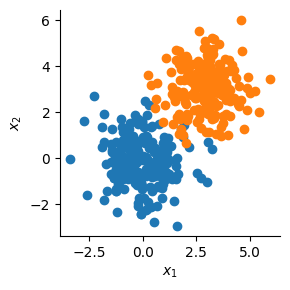
\includegraphics[scale=0.8, max width=\linewidth]{./fig/local-learning-rule/logistic-regression-perceptron/cell006.png}
	\caption{cell006.png}
	\label{cell006.png}
\end{figure}
CSは条件刺激(conditioned stimulus), Rは報酬(reward)を意味する.

この際にprediction error信号の時間的変位(temporal shift)が観察されるが,

\begin{itemize}
\item A gradual temporal shift of dopamine responses mirrors the progression of temporal difference error in machine learning
\end{itemize}
https://www.nature.com/articles/s41593-022-01109-2


Rescorla–Wagner model
